\subsection{Evaluation}
\label{sec:soft_cut_evaluation}

First, we took a closer look at the performance of our three different neural network architectures, we just presented.
Therefore, we compared the accuracy calculated by \textit{caffe} during training.
This corresponds to the per-frame predictions.
To train the neural networks we used our generated data, which is explained in Section~\ref{sec:soft_cut_data_generation}.
The amount of soft cuts and non soft cuts in the training and test data was the same.
We had 2,579,566 training data and 2,412,487 test data.
The accuracy given by \textit{caffe} was the following:
\begin{table}[ht]
	\centering
	\begin{tabular}{l|l}
	CNN + one LSTM                      & 69,80 \% \\ \hline
	CNN + two LSTMs                     & 80,42 \% \\ \hline
	one convolutional layer + two LSTMs & 70,07 \% \\
	\end{tabular}
	\caption{Accuracy of the different neural network architectures given by \textit{caffe}.}
	\label{tab:caffe_accurary}
\end{table}
The \textit{CNN + two LSTMs} has by far the highest accuracy.
Therefore, we decided to take this neural network architecture as our basis for the following evaluations.

Next we evaluated the different merging strategies.
This evaluation was done on the actual video data provided by TrecVid.
We used the frame sequence predictions from the \textit{CNN + two LSTMs} and merged those predictions in the four different ways, presented in the last section (see Figure~\ref{fig:merging_strategies}).
Afterwards, we compared the resulting frame predictions with the actual values (belongs to a soft cut or not) and calculated accuracy, precision, and recall on a frame basis.
The results can be found in Figure~\ref{fig:evaluation_net}.
\begin{figure}[!htb]
	\centering
	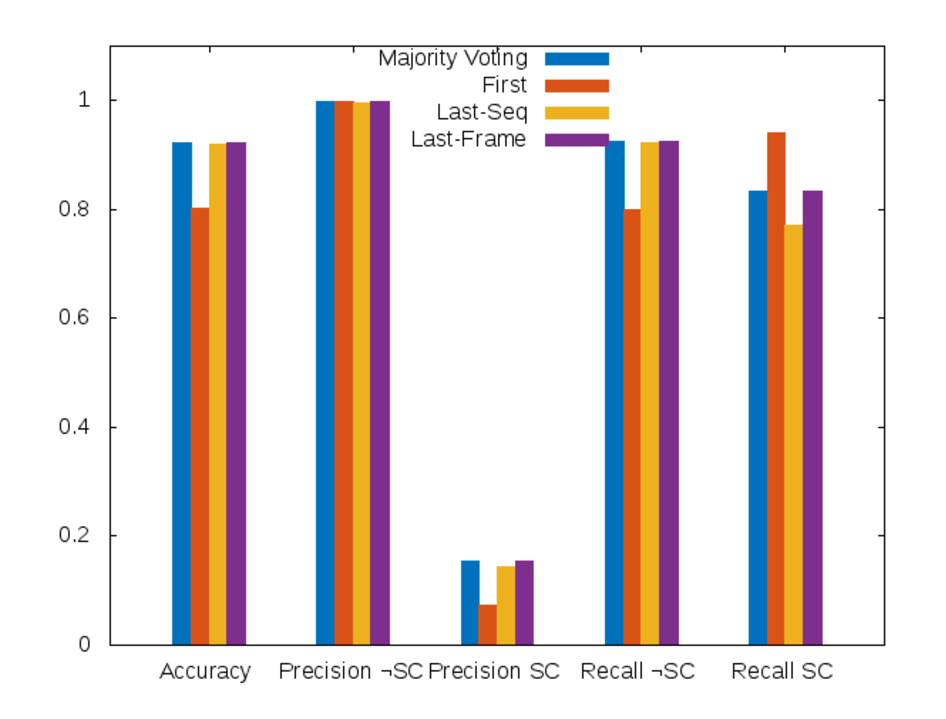
\includegraphics[scale=.7]{images/evalutation_net.eps}
	\caption{Results of the different merging strategies: \textit{Majority-Voting Diagonally} (Majority Voting), \textit{Take First} (First), \textit{Take Last 'Sequence'} (Last-Sequence), \textit{Take Last 'Frame'} (Last-Frame). The \textit{Majority-Voting Diagonally} strategy performs best.}
	\label{fig:evaluation_net}
\end{figure}
As the graphic shows the \textit{Take First} strategy is by far the worst.
The other three strategies perform equally well, but the \textit{Majority-Voting diagonally} is slightly better with an accuracy of 92.29\%.
The recall for both classes (soft cut and non soft cut) is also pretty high: 92.43\% for non soft cuts and 83.46\% for soft cuts.
However, the precision of non soft cuts is almost 100\% for all four strategies, whereas the precision for soft cuts is only around 15\%.
This means, that our deep neural network did not learn, how to recognize soft cuts well.
Only 15\% of the of the predicted frames were soft cuts.
Basically, the deep neural network recognizes almost every frame as non soft cut.

Because we have such a low precision for soft cuts, we also tried to increase the value by trying out the \textit{Gap Filler}.
Unfortunately, this had no impact at all.
The precision of soft cuts did not increase.
Thus, the deep neural network must predict soft cuts, which are not close to other soft cuts and which are at least six frames long.
In those cases the \textit{Gab Filler} will not find any frames.
\textcolor{red}{TODO}

Up to now we used a sequence length of eleven.
Using a sliding window approach to detect soft cuts, we repeatedly test soft cuts of the length eleven.
Having such a low value, allows us to detect parts of a soft cuts, which can afterwards be merged.
If we would have a larger number, it would possible to miss smaller soft cuts.
So, we decided to keep the length such low, so that we do not miss a soft cut.
The average soft cut length in the actual video data is however 21.
Because the results for a sequence length of eleven were not that good, we decided to test our architecture with a sequence length of 21.
Unfortunately, also this did not improve the results.
\textcolor{red}{TODO} %Haben wir dazu überhaupt irgendwelche Ergebnisse?
